\documentclass[11pt,a4paper]{article}
\usepackage[left=2cm, text={17cm,24cm}, top=3cm]{geometry}
\usepackage[czech]{babel}
\usepackage[utf8]{inputenc}
\usepackage{times}
\usepackage[unicode]{hyperref} %pro křížové odkazy
\usepackage{graphicx} %pro práci s obrázky
\usepackage{float}
\usepackage{amsmath} %sazba matematiky
\usepackage{xcolor} %barvičky
\usepackage{listings} %algoritmy, sazba kódu
\usepackage{algpseudocode}
\usepackage{pxfonts}
\usepackage{import}
\usepackage{multicol}
\usepackage{pdflscape}
\usepackage{multicol}
\usepackage{enumitem}
\usepackage{longtable}

\newcommand\Alpha{\mathrm{A}} % Alpha

\lstset{
  language=C,
  numbersep=5pt,
  breaklines=true,  
  breakatwhitespace=false,
  basicstyle=\ttfamily,
  commentstyle=\color{gray},
  keywordstyle=\bfseries,
  showstringspaces=false,
  %numbers=left,
  %numberstyle=\tiny\color{gray},
}

\begin{document}

\begin{titlepage}
    \begin{center}
        
\includegraphics[height = 160pt]{images/FIT_logo.pdf}\\
		
		{\Huge \textsc{Fakulta informačních technologií}\\[5pt]}
		{\Huge \textsc{Vysoké učení technické v~Brně}}\\
		\vspace{\stretch{0.382}}
		{\LARGE Formální jazyky a překladače\\[5pt]}
		{\LARGE Dokumentace k projektu IFJ a IAL\\[30pt]}
		
		\begin{tabular}{c c c c c}
		    \multicolumn{5}{c}{Tým 128, varianta II}\\[5pt]
            \textbf{Jméno} & \textbf{Příjmení} & \textbf{Xlogin} & \textbf{Rozdělení bodů} & \textbf{Role}\\
            \hline
            Michal & Šmahel & xsmahe01 & 47\% & vedoucí týmu \\[5pt]
            Martin & Havlík & xhavli56 & 45\% &\\[5pt]
            Pavel  & Osinek & xosine00 & 8\% & 
        \end{tabular}\\[30pt]
        \textbf{Implementovaná rozšíření:} žádná
    \end{center}
    \vspace{\stretch{0.609}}
    {
		\hfill
		\today
	}
\end{titlepage}

\newpage
\tableofcontents
\newpage

\section{Úvod}
Cílem projektu bylo vytvořit překladač imperativního programovacího jazyka IFJ21, který vychází z jazyka Teal a překládá se do cílového jazyka IFJcode21. Dokumentace má být velmi stručná (v rozsahu 3-5 stran), takže v ní budou uvedeny zpravidla jen zajímavosti z vývoje a strohý popis jednotlivých částí projektu.
        
\section{Implementace překladače}

Tato sekce se bude věnovat samotné práci na překladači. Způsob organizace práce v týmu a další informace lze nalézt v kapitole \ref{sec:team-work}.

    \subsection{Lexikální analýza}
    V první fázi vývoje jsme se věnovali lexikální analýze a pomocným abstraktním datovým typům, které společně s ní využívají i další funkční celky. Klíčový modul spadající do lexikální analýzy je skener. Ten postupně načítá znaky ze standardního vstupu a pomocí konečného automatu (diagramu je věnována podkapitola \ref{sec:fsm-diagram}) sestavuje tokeny, s nimiž se následně pracuje převážně v syntaktické analýze.
    
    Náš skener na doručení z přednášky od doktorky Burgetové rovnou ukládá nově nalezené identifikátory do aktuálně nejlokálnější tabulky symbolů. Během syntaktické analýzy je již kostra tabulky připravená a není je možné s ní rovnou pracovat. Za poznámku jistě stojí zmínka o tom, jak poznáme, zda byla již proměnná deklarována nebo ji jen skener načetl na pravé straně. Tady spoléháme na prostý předpoklad, že deklarovaná proměnná má již u svého identifikátoru uvedeno, že se jedná o proměnnou (nikoliv funkci) a má přidělen typ.
    
    Při tvorbě diagramu jsme využili online simulátoru\cite{fsm-simulator}, který po zadání formální definice automatu generuje ekvivalentní diagram. Tento diagram bylo následně nutné ručně upravit, ale během návrhu konečného automatu nám tento nástroj velmi zpříjemnil práci.
    
        \subsubsection{Diagram konečného automatu}
        \label{sec:fsm-diagram}
        Konečný automat, který je srdcem skeneru, je implementován podle diagramu na obrázku \ref{fig:fsm-diagram}. Pro zvýšení přehlednosti nejsou jednoprvkové množiny přípustných znaků uváděny do složených závorek. Některé rozsáhlejší množiny jsou zastoupeny řeckými písmeny, k nimž se vztahuje následující legenda:
        \begin{itemize}
            \item $\Alpha$ -- znaky A-Z z ASCII tabulky
            \item $\alpha$ -- znaky a-z z ASCII tabulky
            \item $\gamma$ -- znaky 0-9 z ASCII tabulky
            \item $\Sigma$ -- množina všech znaků ASCII tabulky
        \end{itemize}
    
        \begin{figure}[H]
        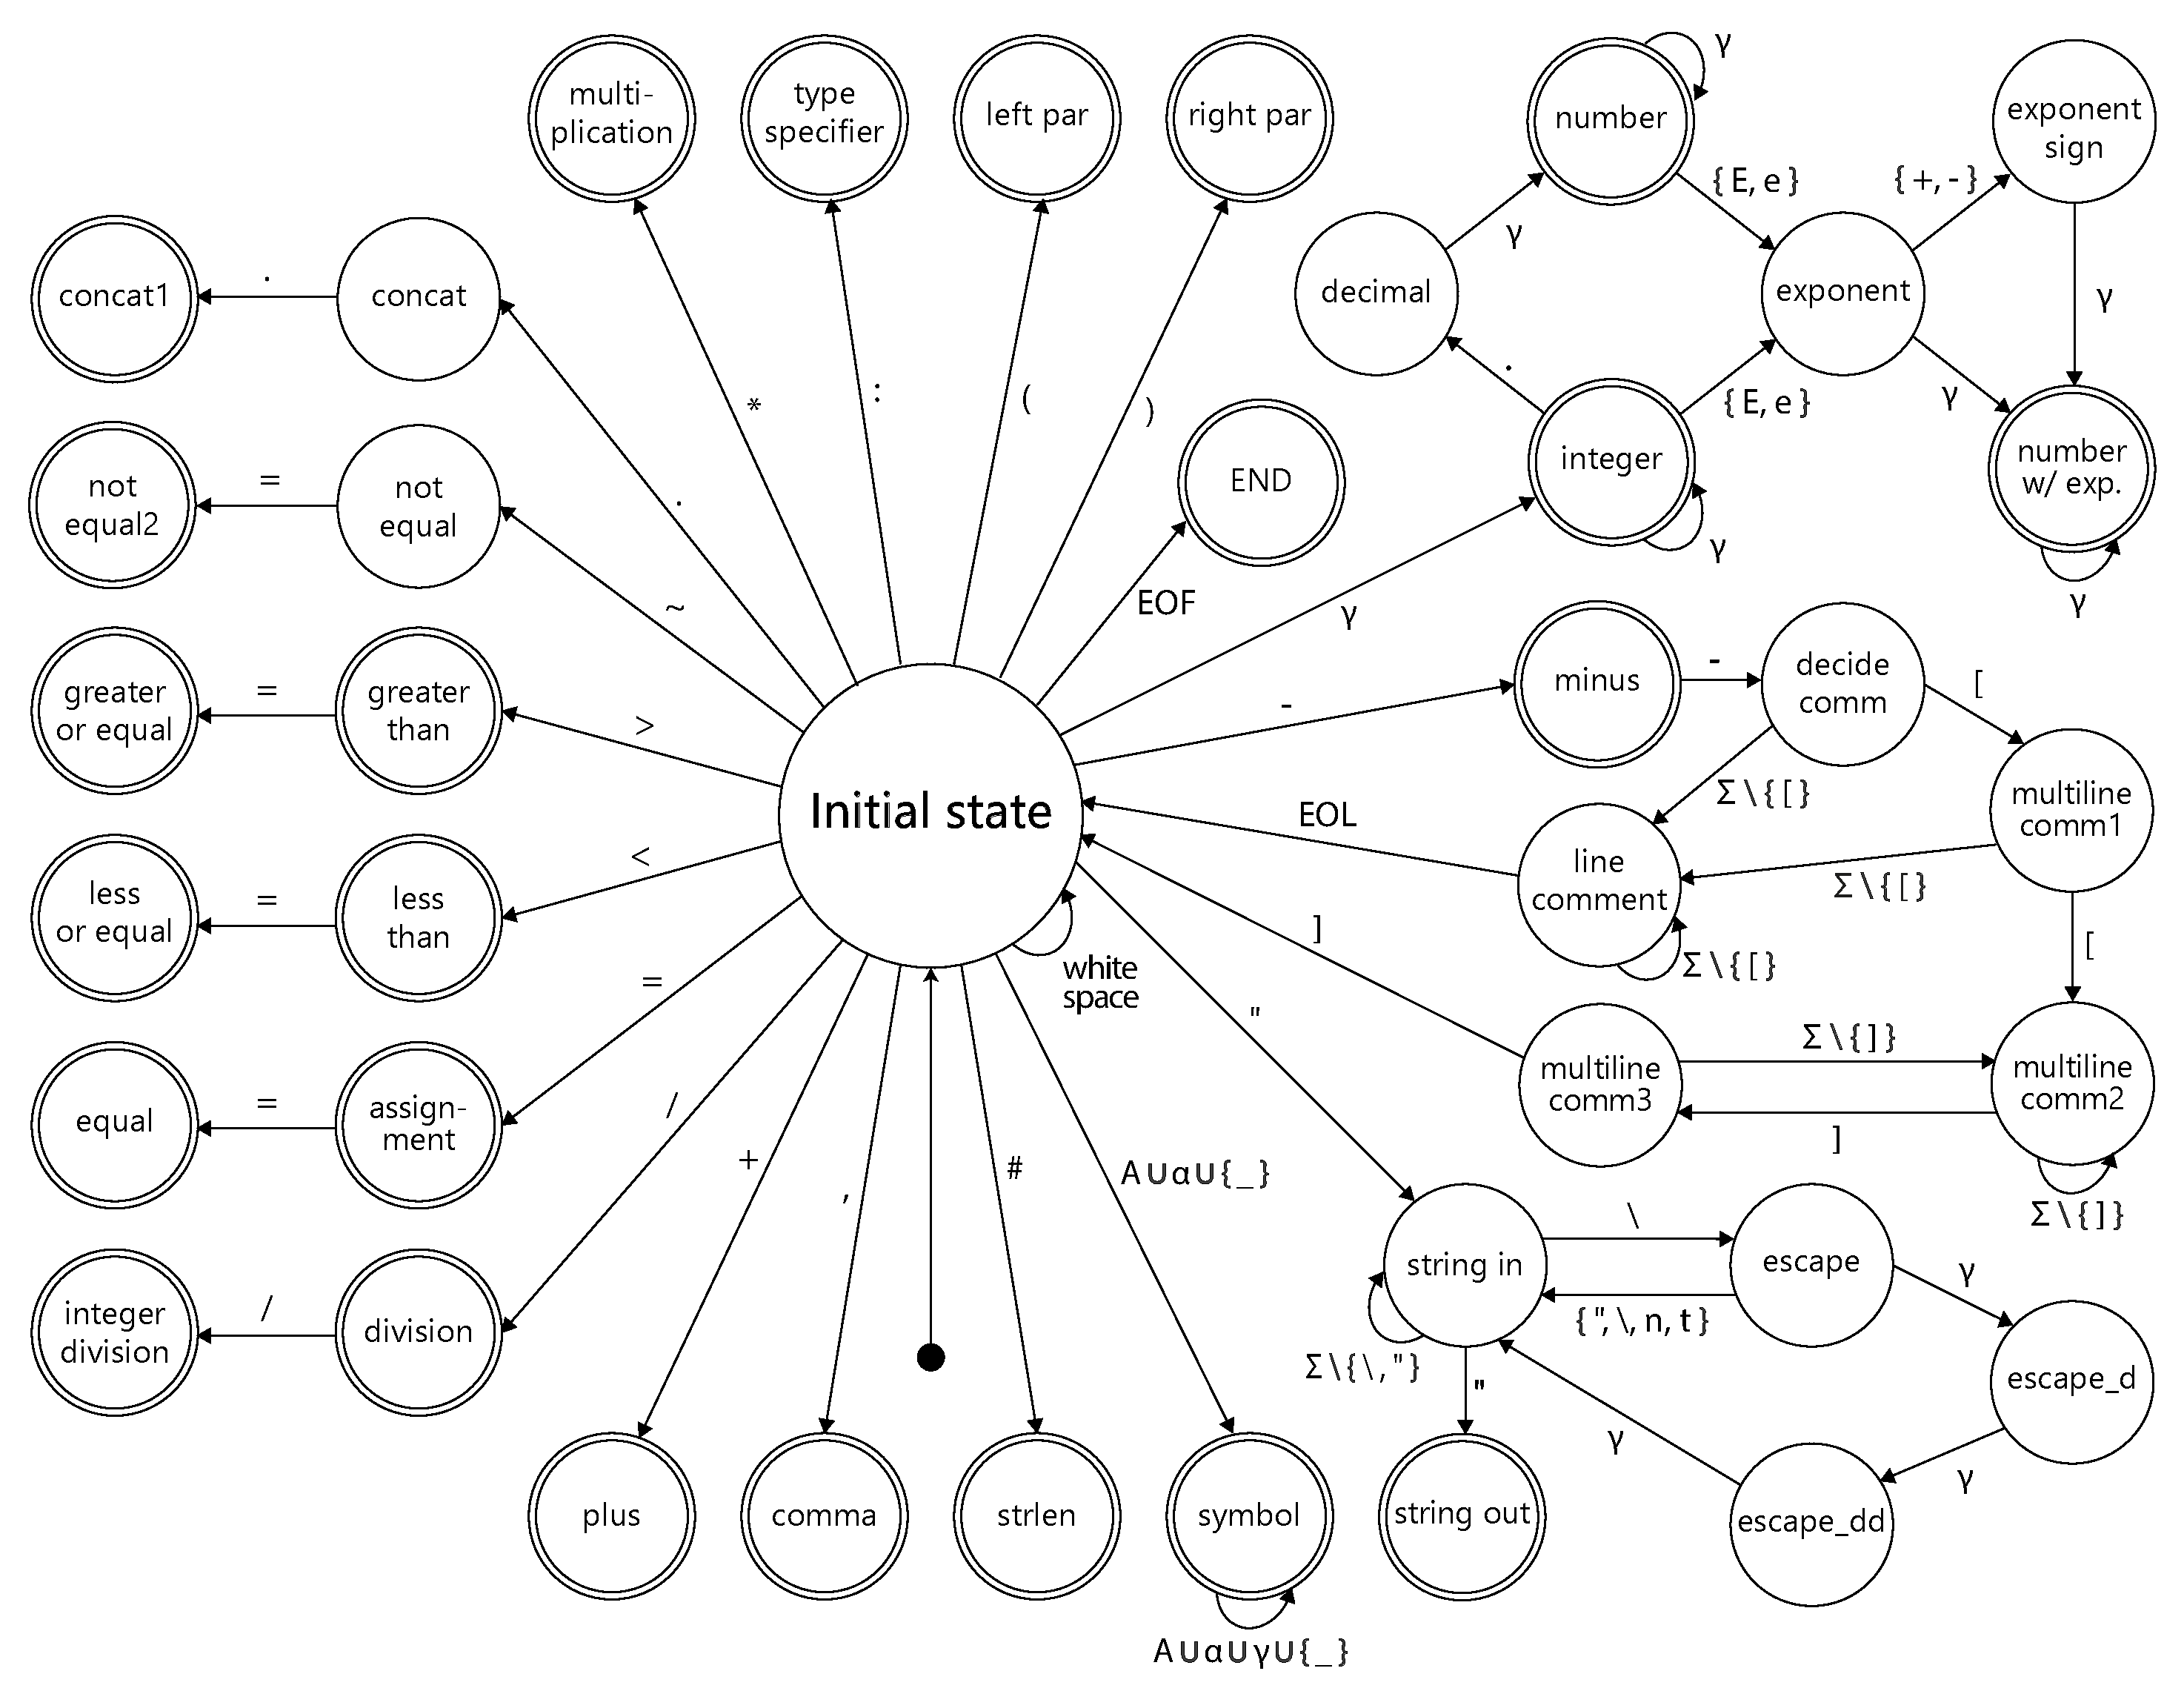
\includegraphics[width=\linewidth]{images/FSM_v11.pdf}
        \caption{Diagram konečného automatu}
        \label{fig:fsm-diagram}
        \end{figure}
    \subsection{Syntaktická analýza}
        \subsubsection{LL-gramatika, SA shora dolů}
        \begin{multicols}{2}
        
        TODO vměstnat sem očíslovaná pravidla gramatiky, já už jsem s tím texem levej, musím to všechno googlit a trvá to, pokud s tím někdo umíte víc, budu rád za pomoc
        \end{multicols}
        Při návrhu LL gramatiky jsme využili online nástroj\cite{LL-grammar-simulator} pro  vizualizaci tvorby derivačního stromu a odzkoušení funkčnosti gramatiky. V implementaci jsme potom zvolili doporučenou metodu rekurzivního sestupu, převážně díky její přímočaré realizaci přepisem z pravidel gramatiky. Implementace se nachází v souboru \texttt{parser.c}.
        
        Porušení LL gramatiky u volání funkcí na pravé straně přiřazení nebo v těle funkce řešíme ukládáním druhu identifikátoru do jej reprezentujícího typu \texttt{identifier\_t}. Potom tedy příchozí token obsahující identifikátor nese informaci zda se jedná o proměnnou/funkci, z čehož rozhodneme, jestli se zanořit do pravidla volání funkce či se přepnout na syntaktickou analýzu zdola nahoru.
        
        \subsubsection{LL-tabulka}
        \begin{table}[ht!]
        \begin{tabular}{|c|c|c|c|c|c|c|c|c|c|c|c|l|}
        \hline
         & \$ & require & global & id & : & function & ( & ) & , & return & end & = \\ \hline
        PROG &  & 1 &  &  &  &  &  &  &  &  &  &  \\ \hline
        REQUIRE &  & 2 &  &  &  &  &  &  &  &  &  &  \\ \hline
        CODE & 4 &  & 3 & 3 &  & 3 &  &  &  &  &  &  \\ \hline
        CODE' &  &  & 5 & 7 &  & 6 &  &  &  &  &  &  \\ \hline
        CODE'' & 9 &  & 8 & 8 &  & 8 &  &  &  &  &  &  \\ \hline
        FUN\_DEC &  &  & 10 &  &  &  &  &  &  &  &  &  \\ \hline
        FUN\_SIGNATURE &  &  &  &  &  & 11 &  &  &  &  &  &  \\ \hline
        TYPE\_LIST &  &  &  &  &  &  &  & 13 &  &  &  &  \\ \hline
        TYPE\_LIST' &  &  &  &  &  &  &  & 15 & 14 &  &  &  \\ \hline
        FUN\_RET & 17 &  & 17 & 17 & 16 & 17 &  &  &  & 17 & 17 &  \\ \hline
        CALL &  &  &  & 18 &  &  &  &  &  &  &  &  \\ \hline
        TERM\_SEQ &  &  &  & 19 &  &  &  & 20 &  &  &  &  \\ \hline
        TERM\_SEQ' &  &  &  &  &  &  &  & 22 & 21 &  &  &  \\ \hline
        FUN\_RET\_LIST &  &  &  &  &  &  &  &  &  &  &  &  \\ \hline
        FUN\_RET\_LIST' & 25 &  & 25 & 25 &  & 25 &  &  & 24 & 25 & 25 &  \\ \hline
        RET\_STMT &  &  &  &  &  &  &  &  &  & 26 &  &  \\ \hline
        RET\_E\_LIST &  &  &  & 28 &  & 29 &  &  &  & 28 & 28 &  \\ \hline
        FUN\_DEF &  &  &  &  &  &  &  &  &  &  &  &  \\ \hline
        PARAM\_LIST &  &  &  & 30 &  &  &  & 31 &  &  &  &  \\ \hline
        PARAM &  &  &  & 32 &  &  &  &  &  &  &  &  \\ \hline
        PARAM' &  &  &  &  &  &  &  & 34 & 33 &  &  &  \\ \hline
        BODY &  &  &  & 35 &  &  &  &  &  & 35 & 36 &  \\ \hline
        BODY' &  &  &  & 38/42 &  &  &  &  &  & 41 & 44 &  \\ \hline
        BODY'' &  &  &  & 43 &  &  &  &  &  & 43 &  &  \\ \hline
        TERM &  &  &  & 45 &  &  &  &  &  &  &  &  \\ \hline
        VAR\_DEC\_DEF &  &  &  &  &  &  &  &  &  &  &  &  \\ \hline
        VAR\_DEC &  &  &  &  &  &  &  &  &  &  &  &  \\ \hline
        TYPE &  &  &  &  &  &  &  &  &  &  &  &  \\ \hline
        VAR\_ASSIGN &  &  &  & 56 &  &  &  &  &  & 56 & 56 & 55 \\ \hline
        STMT &  &  &  & 57 &  &  &  &  &  &  &  &  \\ \hline
        ID\_SEQ &  &  &  & 58 &  &  &  &  &  &  &  &  \\ \hline
        ID\_SEQ' &  &  &  &  &  &  &  &  & 59 &  &  & 60 \\ \hline
        E\_LIST &  &  &  &  &  &  &  &  &  &  &  &  \\ \hline
        E' &  &  &  & 63 &  &  &  &  & 62 & 63 & 63 &  \\ \hline
        IF &  &  &  &  &  &  &  &  &  &  &  &  \\ \hline
        WHILE &  &  &  &  &  &  &  &  &  &  &  &  \\ \hline
        \end{tabular}
        \caption{LL tabulka (1. část)}
    \end{table}

    \begin{table}
        \begin{tabular}{|c|c|c|c|c|c|l|c|c|c|c|c|}
        \hline
         & integer & number & string & nil & local & e & if & then & else & while & do \\ \hline
        PROG &  &  &  &  &  &  &  &  &  &  &  \\ \hline
        REQUIRE &  &  &  &  &  &  &  &  &  &  &  \\ \hline
        CODE &  &  &  &  &  &  &  &  &  &  &  \\ \hline
        CODE' &  &  &  &  &  &  &  &  &  &  &  \\ \hline
        CODE'' &  &  &  &  &  &  &  &  &  &  &  \\ \hline
        FUN\_DEC &  &  &  &  &  &  &  &  &  &  &  \\ \hline
        FUN\_SIGNATURE &  &  &  &  &  &  &  &  &  &  &  \\ \hline
        TYPE\_LIST & 12 & 12 & 12 &  &  &  &  &  &  &  &  \\ \hline
        TYPE\_LIST' &  &  &  &  &  &  &  &  &  &  &  \\ \hline
        FUN\_RET &  &  &  &  & 17 &  & 17 &  &  & 17 &  \\ \hline
        CALL &  &  &  &  &  &  &  &  &  &  &  \\ \hline
        TERM\_SEQ & 19 & 19 & 19 & 19 &  &  &  &  &  &  &  \\ \hline
        TERM\_SEQ' &  &  &  &  &  &  &  &  &  &  &  \\ \hline
        FUN\_RET\_LIST & 23 & 23 & 23 &  &  &  &  &  &  &  &  \\ \hline
        FUN\_RET\_LIST' &  &  &  &  & 25 &  & 25 &  &  & 25 &  \\ \hline
        RET\_STMT &  &  &  &  &  &  &  &  &  &  &  \\ \hline
        RET\_E\_LIST &  &  &  &  & 28 & 27 & 28 &  & 28 & 28 &  \\ \hline
        FUN\_DEF &  &  &  &  &  &  &  &  &  &  &  \\ \hline
        PARAM\_LIST &  &  &  &  &  &  &  &  &  &  &  \\ \hline
        PARAM &  &  &  &  &  &  &  &  &  &  &  \\ \hline
        PARAM' &  &  &  &  &  &  &  &  &  &  &  \\ \hline
        BODY &  &  &  &  & 35 &  & 35 &  & 36 & 35 &  \\ \hline
        BODY' &  &  &  &  & 37 &  & 39 &  &  & 40 &  \\ \hline
        BODY'' &  &  &  &  & 43 &  & 43 &  & 44 & 43 &  \\ \hline
        TERM & 46 & 47 & 48 & 49 &  &  &  &  &  &  &  \\ \hline
        VAR\_DEC\_DEF &  &  &  &  & 50 &  &  &  &  &  &  \\ \hline
        VAR\_DEC &  &  &  &  & 51 &  &  &  &  &  &  \\ \hline
        TYPE & 52 & 53 & 54 &  &  &  &  &  &  &  &  \\ \hline
        VAR\_ASSIGN &  &  &  &  & 56 &  & 56 &  & 56 & 56 &  \\ \hline
        STMT &  &  &  &  &  &  &  &  &  &  &  \\ \hline
        ID\_SEQ &  &  &  &  &  &  &  &  &  &  &  \\ \hline
        ID\_SEQ' &  &  &  &  &  &  &  &  &  &  &  \\ \hline
        E\_LIST &  &  &  &  &  & 61 &  &  &  &  &  \\ \hline
        E' &  &  &  &  & 63 &  & 63 &  & 63 & 63 &  \\ \hline
        IF &  &  &  &  &  &  & 64 &  &  &  &  \\ \hline
        WHILE &  &  &  &  &  &  &  &  &  & 65 &  \\ \hline
        \end{tabular}
        \caption{LL tabulka (1. část)}
    \end{table}
        
        \subsection{SA zdola nahoru}
        \subsubsection{Precedenční tabulka}
        
        \begin{table}[ht]
        \begin{tabular}{|c|c|c|c|c|c|c|c|c|c|c|c|c|c|c|c|c|c|}
        \hline
         & \# & * & / & // & + & - & .. & \textless{} & \textless{}= & \textgreater{} & \textgreater{}= & == & $\sim$= & ( & ) & term & \$ \\ \hline
        \# &  & \textgreater{} & \textgreater{} & \textgreater{} & \textgreater{} & \textgreater{} & \textgreater{} & \textgreater{} & \textgreater{} & \textgreater{} & \textgreater{} & \textgreater{} & \textgreater{} & \textless{} & \textgreater{} & \textless{} & \textgreater{} \\ \hline
        * & \textless{} & \textgreater{} & \textgreater{} & \textgreater{} & \textgreater{} & \textgreater{} & \textgreater{} & \textgreater{} & \textgreater{} & \textgreater{} & \textgreater{} & \textgreater{} & \textgreater{} & \textless{} & \textgreater{} & \textless{} & \textgreater{} \\ \hline
        / & \textless{} & \textgreater{} & \textgreater{} & \textgreater{} & \textgreater{} & \textgreater{} & \textgreater{} & \textgreater{} & \textgreater{} & \textgreater{} & \textgreater{} & \textgreater{} & \textgreater{} & \textless{} & \textgreater{} & \textless{} & \textgreater{} \\ \hline
        // & \textless{} & \textgreater{} & \textgreater{} & \textgreater{} & \textgreater{} & \textgreater{} & \textgreater{} & \textgreater{} & \textgreater{} & \textgreater{} & \textgreater{} & \textgreater{} & \textgreater{} & \textless{} & \textgreater{} & \textless{} & \textgreater{} \\ \hline
        + & \textless{} & \textless{} & \textless{} & \textless{} & \textgreater{} & \textgreater{} & \textgreater{} & \textgreater{} & \textgreater{} & \textgreater{} & \textgreater{} & \textgreater{} & \textgreater{} & \textless{} & \textgreater{} & \textless{} & \textgreater{} \\ \hline
        - & \textless{} & \textless{} & \textless{} & \textless{} & \textgreater{} & \textgreater{} & \textgreater{} & \textgreater{} & \textgreater{} & \textgreater{} & \textgreater{} & \textgreater{} & \textgreater{} & \textless{} & \textgreater{} & \textless{} & \textgreater{} \\ \hline
        .. & \textless{} & \textless{} & \textless{} & \textless{} & \textless{} & \textless{} & \textless{} & \textgreater{} & \textgreater{} & \textgreater{} & \textgreater{} & \textgreater{} & \textgreater{} & \textless{} & \textgreater{} & \textless{} & \textgreater{} \\ \hline
        \textless{} & \textless{} & \textless{} & \textless{} & \textless{} & \textless{} & \textless{} & \textless{} &  &  &  &  &  &  & \textless{} & \textgreater{} & \textless{} & \textgreater{} \\ \hline
        \textless{}= & \textless{} & \textless{} & \textless{} & \textless{} & \textless{} & \textless{} & \textless{} &  &  &  &  &  &  & \textless{} & \textgreater{} & \textless{} & \textgreater{} \\ \hline
        \textgreater{} & \textless{} & \textless{} & \textless{} & \textless{} & \textless{} & \textless{} & \textless{} &  &  &  &  &  &  & \textless{} & \textgreater{} & \textless{} & \textgreater{} \\ \hline
        \textgreater{}= & \textless{} & \textless{} & \textless{} & \textless{} & \textless{} & \textless{} & \textless{} &  &  &  &  &  &  & \textless{} & \textgreater{} & \textless{} & \textgreater{} \\ \hline
        == & \textless{} & \textless{} & \textless{} & \textless{} & \textless{} & \textless{} & \textless{} &  &  &  &  &  &  & \textless{} & \textgreater{} & \textless{} & \textgreater{} \\ \hline
        $\sim$= & \textless{} & \textless{} & \textless{} & \textless{} & \textless{} & \textless{} & \textless{} &  &  &  &  &  &  & \textless{} & \textgreater{} & \textless{} & \textgreater{} \\ \hline
        ( & \textless{} & \textless{} & \textless{} & \textless{} & \textless{} & \textless{} & \textless{} & \textless{} & \textless{} & \textless{} & \textless{} & \textless{} & \textless{} & \textless{} & = & \textless{} &  \\ \hline
        ) &  & \textgreater{} & \textgreater{} & \textgreater{} & \textgreater{} & \textgreater{} & \textgreater{} & \textgreater{} & \textgreater{} & \textgreater{} & \textgreater{} & \textgreater{} & \textgreater{} &  & \textgreater{} &  & \textgreater{} \\ \hline
        term &  & \textgreater{} & \textgreater{} & \textgreater{} & \textgreater{} & \textgreater{} & \textgreater{} & \textgreater{} & \textgreater{} & \textgreater{} & \textgreater{} & \textgreater{} & \textgreater{} &  & \textgreater{} &  & \textgreater{} \\ \hline
        \$ & \textless{} & \textless{} & \textless{} & \textless{} & \textless{} & \textless{} & \textless{} & \textless{} & \textless{} & \textless{} & \textless{} & \textless{} & \textless{} & \textless{} &  & \textless{} &  \\ \hline
        \end{tabular}
        \end{table}
    
    \subsection{Sémantická analýza}
    Sémantické kontroly a akce jsme vpisovali přímo do jednotlivých funkcí rekurzivního sestupu SA shora dolů a do funkcí představující aplikovaná pravidla v SA zdola nahoru.
    
    \subsection{Generátor cílového kódu}
    Jelikož si žádnou vnitřní reprezentaci kódu nevytváříme, cílový kód generujeme rovnou při analýze. To znamená pár ústupků efektivnímu (generování) kódu:
    \begin{itemize}
        \item Vestavěné funkce generujeme v jednom bloku, který přeskočíme, na začátku cílového kódu
        \item Každý kód těla funkce je též obalen skokem přes něj
        \item Výpočty výrazů provádíme pomocí zásobníkových instrukcí s využitím přirozeného postfixového zpracování SA zdola nahoru
    \end{itemize}
    
    \subsection{Tabulka symbolů}
    Pro naši variantu jsme implementaci pomocí tabulky s rozptýlenými položkami převzali z domácího úkolu z předmětu IJC. Jako položku tabulky jsme vytvořili strukturu \texttt{identifier\_t} uchovávající potřebné informace o identifikátoru. Mezi ukládané informace patří název, pozice ve vstupním kódu pro jednoznačné pojmenování, typ (proměnná/funkce) a dále specifické informace pokud se jedná o proměnnou, zejména její typ, nebo pokud se jedná o funkci, kde nejdůležitější je její signatura.
    
    Pro rozsahy platnosti proměnných využíváme \texttt{symstack\_t}, zásobníkový ADT, do kterého si ukládáme ukazatele na nově vzniklé lokální tabulky symbolů pro každý začínající blok a ze kterého je opět odstraňujeme na konci bloku. Při vyhledávání proměnné prohledáme nejlokálnější tabulku symbolů, při nenalezení získáme ze \texttt{symstack\_t} nadřazenou tab. symb., opět prohledáme atd.
    
    \subsection{Implementovaná rozšíření}
    
    Implementace rozšíření nás sice původně lákala, ale nakonec na tuto fázi projektu nezbyl čas, jelikož jsme řešili projekt víceméně ve dvou lidech s občasnými drobnými příspěvky třetího člena. Podrobněji se této problematice věnuje kapitola \ref{sec:tasks-division}.
    
% \newpage
\section{Práce v týmu}
\label{sec:team-work}

V této kapitole bych z pozice vedoucího týmu rád popsal, jakým způsobem fungoval náš tým, uvedl pár informací k organizaci práce v týmu, dělení úkolů a přidělování bodových částí.

\subsection{Způsob práce na projektu}
\label{sec:way-to-work-on-project}

Na projektu měli pracovat všichni členové týmu. Projekt byl rozdělen na větší množství menších podproblémů s různou mírou složitosti. Rozdělení do úkolů, jejich správu a dohled nad jejich řešením měl na starost vedoucí týmu. O tom, jaký úkol bude kdo vypracovávat však nebylo explicitně rozhodováno, každý člen si mohl zvolit, na čem bude v danou chvíli pracovat. Byla snaha rozdělit úkoly do minimalistických celků, aby se každý člen týmu mohl podílet na řešení každé části vývoje kompilátoru, pokud by měl zájem. Jako příklad lze uvést fakt, že byl každý pomocný abstraktní datový typ vyčleněn do samostatného úkolu.

Cílem bylo, aby měl každý člen alespoň základní povědomí o všech částech projektu. Kvůli tomu, že na jednom větším celku (např. lexikální analýza) pracovalo větší množství lidí, byla také podněcována jejich vzájemná komunikace, při níž bylo třeba domlouvat rozhraní mezi jednotlivými moduly. Nebyl tedy zvolen postup, kdy se rozdělí větší celky a poté se provádí jejich kompozice.

\subsection{Využité nástroje a procesy}

Kvůli jednoduší spolupráci na tvorbě projektu jsme se rozhodli využít verzovací systém Git se vzdáleným repozitářem hostovaným službou Github. Na této službě jsme kromě funkce vzdáleného repozitáře pro správu verzí projektu využili také několik dalších funkcí, které budou popsány v dalších odstavcích.

Github nabízí možnost vytvořit si projekt, který se naváže na repozitáře a umožňuje zřídit automatizované plánování úkolů metodou Kanban, která spočívá v rozdělování úkolů do několika fází. Mezi tyto fáze patří \uv{Naplánováno} (\uv{Backlog} nebo \uv{To do}), kde jsou naplánované úkoly, na nichž zatím nikdo nepracuje; \uv{V procesu} (\uv{In progress}) s rozpracovanými úkoly a \uv{Hotovo} (\uv{Done}), která obsahuje dokončené úkoly. Kromě těchto základních fází jsme používali ještě některé rozšířené pro označení stavu revizí požadavků na začlenění změn. Díky tomu bylo možné na jedné obrazovce vidět, jak si tým stojí a v jakém stavu rozpracování aktuálně projekt je.

Služba Github poskytuje různé možnosti omezení přístupu k větvím a určitým typům změn. Díky tomu bylo možné uzamknout výchozí větev a pro veškeré změny vynucovat revize od jiného člena týmu. Autor změn tak vždy dostal zpětnou vazbu od někoho dalšího a podařilo se tak odhalit mnoho chyb, kterých si autor nevšiml. Začleňování změn do hlavní větve bylo prováděno výhradně pomocí webového rozhraní pro žádosti o začlenění změn (běžněji známo pod anglickým pojmem \uv{pull request}). Tam je možné změny komentovat a navrhovat různé úpravy a opravy chyb nalezených během revize.

Poslední důležitou funkcí poskytovanou Githubem je Github Actions. Tato funkce umožňuje automatické spouštění testů a různých akcí využívajících Github API pro správu repozitářů a projektů. Díky tomu bylo možné automaticky spouštět testy pro veškeré provedené změny, díky čemuž jsme měli vždy přehled o tom, jestli změna nerozbíjí dříve implementované funkcionality apod. Navíc jsme díky sadě pravidel docílili úplné automatizace Kanban fází, takže nebylo nutné mezi nimi úkoly ručně přesouvat. To zamezilo vzniku chyb a zobrazený přehled vždy reflektovat aktuální stav projektu.

Samotné psaní kódu si pak členové týmu zařídili po svém podle toho, co komu vyhovovalo. K dispozici byla poměrně komplexní konfigurace nástroje Make, která poskytovala automatickou kompilaci a sestavování zdrojových kódů, jednotkových a manuálních testů, přípravu výsledného archivu pro odevzdání a další drobnosti.

\subsection{Rozdělení úkolů}
\label{sec:tasks-division}

Jak bylo zmíněno v kapitole \ref{sec:way-to-work-on-project}, členové týmu si mohli sami volit, čemu se budou věnovat. Jelikož se některé větší úkoly dále špatně dělí, každý člen se nakonec některým částem vývoje kompilátoru věnoval více než jiným, a s trochou nadsázky by se dalo říct, že se na ně \uv{specializoval}. V následujících odstavcích bude rozvedeno rozdělení klíčových částí mezi členy projektu.

Lexikální analýze se primárně věnoval Michal Šmahel. Tato část byla však značně rozdělena i mezi další členy týmu, kteří spolupracovali na pomocných implementacích. Diagram lexikální analýzy (viz obrázek č. \ref{fig:fsm-diagram}) skládali všichni členové týmu na prezenční schůzce. Dále se vytvářely různé pomocné datové struktury, kterým se mimo Michala Šmahela věnoval i Martin Havlík a částečně také Pavel Osinek.

Syntaktická a sémantická analýza byla rozdělena mezi Michala Šmahela a Martina Havlíka. Zpracování struktury zdrojových souborů pomocí metody shora dolů se ujal Martin Havlík, zpracování výrazů metodou zdola nahoru se poté zabýval Michal Šmahel. Ten však řešil pouze implementaci, precedenční tabulku skládal Martin Havlík. Sémantické kontroly a akce následně doplňoval každý do svého modulu sám.

Generování kódu se věnoval opět Michal Šmahel s Martinem Havlíkem. Základní principy generování vymýšleli na týmových schůzkách, kam většinou Pavel Osinek z různých důvodů nedocházel. Implementaci hlavní části následně provedl Martin Havlík s drobnými zásahy (převážně optimalizace generovaného kódu) od Michala Šmahela. Ten kromě toho kompletně vypracoval generování kódu pro vestavěné funkce.

Michal Šmahel se dále, coby vedoucí týmu, podílel na organizaci práce a dohledu na ostatní členy týmu. Rovněž se významně podílel a přípravě pracovního prostředí a testů. Pavel Osinek připravoval šablonu dokumentace a grafickou podobu diagramu stavového automatu.

Důvodem, proč tato kapitola nabývá nadměrné délky, je problém s jedním členem týmu, který se rozhodl projektu věnovat minimum času a úsilí, což bylo nutné dále řešit nerovnoměrným rozdělením bodů. Kvůli této záležitosti byl osloven i dr. Křivka, který povolil výrazné snížení bodů Pavlu Osinkovi, pokud bude dostatečně prokazatelné, kdo měl na čem jaký podíl. Dohodli jsme se na zavedení bodového systému k úkolům zmíněným v kapitole \ref{sec:way-to-work-on-project}, podle něhož se následně spočítala procenta a po drobné korekci v řádu malých jednotek procent prohlásila za finální rozdělení bodů. Doufám, že tato kapitola splnila svůj účel a dokreslila, jakým způsobem se jednotliví členové na projektu podíleli a výsledné bodové rozdělení je tím dostatečně odůvodněné. V případě problémů jsou je k dispozici historie úkolů a jejich bodování včetně automatického hodnotícího skriptu.

\section{Vývoj}
\section{Závěr}

\newpage

\section{Zdroje}
    \bibliographystyle{czechiso}
    \bibliography{references}

%     Zkouška citace~\cite{MedunaAlexander2008Eocd}.
    
%     Ukázka \uv{českých} uvozovek.
    
%     Ukázka kódu
%     \begin{lstlisting}
% #include <stdio.h>

% int main() {
%     // printf() displays the string inside quotation
%     printf("Hello, World!");
%     return 0;
% }\end{lstlisting}
          
%     \begin{algorithmic}
%         \State $i \gets 10$
%         \If{$i\geq 5$} 
%             \State $i \gets i-1$
%         \Else
%             \If{$i\leq 3$}
%                 \State $i \gets i+2$
%             \EndIf
%         \EndIf 
%     \end{algorithmic}        

\end{document}
